\section{Pianificazione} \label{section:pianificazione}

Considerate le scadenze indicate in \hyperref[subsection:intro_scadenze]{1.5 Scadenze}, si è deciso di organizzare lo sviluppo del progetto nei seguenti periodi:
\begin{itemize}
    \item \textbf{Analisi preliminare};
    \item \textbf{Progettazione Technology Baseline};
    \item \textbf{Codifica Proof of Concept};
    \item \textbf{Progettazione di dettaglio e codifica requisiti obbligatori};
    \item \textbf{Progettazione di dettaglio e codifica requisiti opzionali};
    \item \textbf{Validazione e collaudo}.
  \end{itemize}
Per una maggiore comprensione, la suddivisione dei periodi lungo la linea temporale viene riassunta graficamente tramite la seguente sequenza temporale:
\begin{figure}[H]
 \centering
  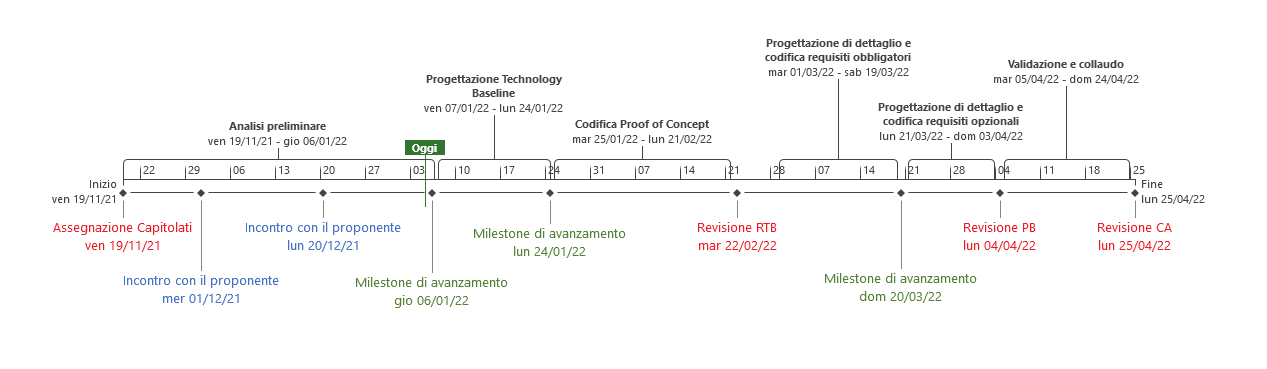
\includegraphics[scale=0.6]{immagini/sequenza_temporale.png}
  \caption{Panoramica della sequenza temporale}
\end{figure}
Il periodo di sviluppo del prodotto è suddiviso in periodi incrementali prefissati. Ogni periodo viene suddiviso in attività, le quali possono essere a loro volta scomposte in sotto-attività più dettagliate.
Le scadenze temporali di alcuni incrementi sono state scelte in base alle revisioni di avanzamento, in modo che il sistema possa evolvere in base ai feedback ricevuti.
Per rappresentare temporalmente le attività viene utilizzato un diagramma di Gantt.
\\Le attività possono essere dei seguenti tipi:
\begin{itemize}
    \item \textbf{Attività critiche:} attività particolarmente importanti per il corretto sviluppo del progetto. La loro data di fine non è slittabile e il ritardo di una di esse
    incide gravemente sulle altre, causando ritardi a cascata. Sono indicate con il colore rosso;
    \item \textbf{Attività non critiche:} attività di minore importanza dalle quali non dipende lo sviluppo generale del progetto. La loro data di fine può essere slittata e non causerebbe ritardi a cascata.
    Sono indicate con il colore blu;
    \item \textbf{Attività di verifica:} attività poste alla fine dei vari periodi per garantire un controllo sulle altre attività svolte.
    Sono indicate con il colore verde;
    \item \textbf{Evento prefissato:} rappresenta un particolare evento di durata pari a zero giorni. Può rappresentare una milestone interna (rombo di colore verde), la consegna dei documenti
    per una revisione, una revisione di avanzamento (rombo di colore rosso) oppure un incontro con il
    proponente (rombo di colore blu). Sono indicate con un rombo colorato.
  \end{itemize}
%%%%%%%%%%%%%%%%%%%%%%%%%%%%%%%%%%%%%%%%%%%%%%%%%%%%%%%%%%%%%%

\subsection{Requirements and Technology Baseline} \label{subsection:pianificazione_rtb}
\subsubsection{Obiettivi} \label{subsubsection:obiettivi_rtb}
\subsubsection{Periodi e attività} \label{subsubsection:periodi_rtb}

%%%%%%%%%%%%%%%%%%%%%%%%%%%%%%%%%%%%%%%%%%%%%%%%%%%%%%%%%%%%%%

\subsection{Product Baseline} \label{subsection:pianificazione_pb}
\subsubsection{Obiettivi} \label{subsubsection:obiettivi_pb}
\subsubsection{Periodi e attività} \label{subsubsection:periodi_pb}

%%%%%%%%%%%%%%%%%%%%%%%%%%%%%%%%%%%%%%%%%%%%%%%%%%%%%%%%%%%%%%

\subsection{Customer Acceptance} \label{subsection:pianificazione_ca}
\subsubsection{Obiettivi} \label{subsubsection:obiettivi_ca}
\subsubsection{Periodi e attività} \label{subsubsection:periodi_ca}